% Hierarchical diagrams, DBDA
% ---------------------------------
% Tinu Schneider, October 2013


\documentclass[12pt]{article}

\usepackage[T1]{fontenc} 
\usepackage[utf8]{inputenc}

\usepackage[margin = 20mm, nohead, nofoot]{geometry} 

\usepackage{tikz}
    \usetikzlibrary{positioning, arrows, backgrounds, decorations, shapes,
    				decorations.pathmorphing, decorations.markings}
  
\graphicspath{{./MiniPlots/}}
    
\pagestyle{empty}

\usepackage{tgheros} 
\renewcommand*\familydefault{\sfdefault} 
	

% Macros for the distributions
% greek
\newcommand{\normalGreek}[2]{\funGreek{#1}{#2}{N}{Normal}} 
\newcommand{\gammaGreek} [2]{\funGreek{#1}{#2}{G}{Gamma}}   

\newcommand{\funGreek}[4]{$\mathcal{#3}$\large$(#1, #2)$ \includegraphics[scale = 0.25]{#4.png} }				 	 
   			
% letters (constants)  
\newcommand{\normalLetters}[2]{\funLetters{#1}{#2}{N}{Normal}} 
\newcommand{\gammaLetters} [2]{\funLetters{#1}{#2}{G}{Gamma}}   

\newcommand{\funLetters}[4]{$\mathcal{#3}(#1, #2)$ \includegraphics[scale = 0.25]{#4.png} }	


% Macros to place symbols and distros
\newcommand{\placeSymbol}[3]{ % 1: symbol, 2: parent-node 3: name of this node
		\node[symbol, yshift = 0.20cm] at (#2.north) (#3) {#1};
	}
\newcommand{\placeDistro}[3]{ % 1: name ot the distro, 2: parent-node, 3: name of this node
		\node[distro, yshift = -0.25cm] at (#2.south) (#3) { \includegraphics[scale = 0.25]{#1.png}};
	}  						 	
   						 	
   						 	  						 	 
\begin{document} % ------------------------------ %

% distances
\def\smallY{0.25}
\def\midY{2.25}

\def\smallX{1.2}
\def\midX{1.5}
\def\bigX{2.7}


\begin{tikzpicture}[ framed,
   	node distance = \midY cm,  on grid,
   	inner frame xsep = 2ex,
   	inner frame ysep = 3ex,
    	box/.style = { rectangle, 
	       		%draw,
	       		rounded corners, 
	       		color = lightgray, 
	       		text = black,  
	       		inner sep = 0pt, 
	       		minimum width = \midX cm,
	       		text width = 2.5cm, 
	       		align = center},
       	boxLegend/.style = {align = left, text width = 4cm, xshift = 2.2cm, 
       				yshift = 1.2cm,  font = \scriptsize, color = black!70},
       	symbol/.style = {box, font = \large, inner sep = 0pt},
       	distro/.style = {inner sep = 0pt},
       	centerpoint/.style = {circle, inner sep = 1pt, blue},
    	allArrows/.style = {font = \footnotesize, color = black!80, text = black},
    	arrSnake/.style = {allArrows, >=stealth', ->, shorten >= 3pt, line join = round, decorate, 
  				decoration={snake, segment length = 10, amplitude = 1.2,
        					post = lineto, post length = 4pt} },
     	implies/.style  = {allArrows, -implies, double, double equal sign distance, shorten >= 0pt}, 
     	labArrow/.style = {pos = 0.36},
     	labArrowLegend/.style = {labArrow, above, font = \tiny, inner sep = 3pt}
  	] 		   		
   		
   	% 'Boxes' for the distributions	and equation(s)
   	% starting at the bottom				
	\node [box] (yij) {\Large $y_{j|i}$};

   	\node [box, above = of yij, yshift = -0.2cm] (omega) {\normalGreek{\omega_{j|i}}{\lambda} } ;
   	
   	\node [box, above = of omega, xshift=-\smallX cm] (linMod)   
   			{ \large $ \underbrace{\varphi_i + \xi_i \cdot x_{j|i}}{}$ } ;
    	
   	\node [box, above = of omega,  xshift =  \bigX cm] (proLambda) {\gammaLetters{K}{I} } ;
    	
    	
   	% Example for 'double nodes'
   	% upper for the symbols / letters
   	% lower for the distrogram
   	\node[centerpoint, above = of linMod, xshift = -\bigX cm] (proPhiCenter) {};
 	   	\placeSymbol{$\kappa,\ \delta$}{proPhiCenter}{proPhiPars}
 		\placeDistro{Normal}{proPhiCenter}{proPhiDistro}
   	%\node [box, above = of linMod, xshift = -\bigX cm]   (proPhi)   { 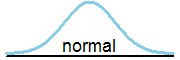
\includegraphics[scale = 0.25]{Normal.png} };
   	\node [box, above = of linMod, xshift =  \bigX cm]   (proXi)    {\normalGreek{\zeta}{\gamma} } ;
   	
   	\node [box, above = of proPhiCenter, xshift = -\smallX cm] (proKappa) {\normalLetters{M}{H} } ;
   	\node [box, above = of proPhiCenter, xshift =  \smallX cm] (proDelta) {\gammaLetters{K}{I} } ;    
   	
   	\node [box, above = of proXi,  xshift = -\smallX cm] (proZeta)  {\normalLetters{M}{H} } ;
   	\node [box, above = of proXi,  xshift =  \smallX cm] (proGamma) {\gammaLetters{K}{I} } ;  
   	
   	
   	% Example for a 'double node'
   	% upper for the symbols / letters
   	% lower for the distrogram
   	% with a 'centerpoint' as anchor
   	\node[centerpoint, above = of linMod, xshift = -\bigX cm] (proPhiCenter) {};
   		\placeSymbol{$\kappa,\ \delta$}{proPhiCenter}{proPhiPars}  % upper
   		\placeDistro{Normal}{proPhiCenter}{proPhiDistro}  % lower
   		    	
   		    	
   	% Arrows	    	
   	\draw[arrSnake] (omega.south) --  node[right, labArrow] {$j|i$} (yij);
   	
       \draw[implies]  (linMod.south) -- node[right, labArrow] {$\ j|i$} (omega.110);
       
        \draw[arrSnake] (proLambda.south) -- (omega.38);   
        
        \draw[arrSnake] (proPhiDistro.south) -- node[right, labArrow] {$\ i$} (linMod.160);       	 	
        \draw[arrSnake] (proXi.south) --  node[left, labArrow]  {$i\quad $} (linMod.75); 
             	
        \draw[arrSnake] (proKappa.south) -- (proPhiPars.145);       	 	
        \draw[arrSnake] (proDelta.south) -- (proPhiPars.35);  
        
        \draw[arrSnake] (proZeta.south) -- (proXi.110);       	 	
        \draw[arrSnake] (proGamma.south) -- (proXi.49);    	
   	
   	
  	% Legend; needs improvement...
   	\node [boxLegend] at ( current bounding box.south west) (legendTitle) 
   		{%
   		\begin{tabular}{ll}
   			$A, \dots, Z$  & Constants \\
   			$a, \dots, z$ & Variables \\
   			$\alpha, \dots, \omega$ & Parameters \\ %[1ex]
   			
			 & deterministic \\[-0.4ex]
			 & relation \\ %[1ex]
			 
			 & stochastic \\[-0.4ex]
			 & relation \\ %[1ex]
			 
			\multicolumn{2}{l}{$i, j = 1, 2, 3, \dots $} \\
   		\end{tabular}
   	};
   				
   	\def\xLegendArrowLeft{-6}
   	\def\xLegendArrowRight{-4.7}  
   	 	
   	\def\yLegendDouble{0.95}
   	\def\yLegendSnake{0.35}
   	
   	\draw[implies, black!70]  (\xLegendArrowLeft, \yLegendDouble) -- (\xLegendArrowRight, \yLegendDouble);    	   	
    \draw[arrSnake, black!70] (\xLegendArrowLeft, \yLegendSnake) -- (\xLegendArrowRight, \yLegendSnake);    	

\end{tikzpicture}

\end{document} % ------------------------------ %
